\documentclass[11pt]{article}
\usepackage[utf8]{inputenc} % Para caracteres en español
\usepackage{amsmath,amsthm,amsfonts,amssymb,amscd}
\usepackage{multirow,booktabs}
\usepackage[table]{xcolor}
\usepackage{fullpage}
\usepackage{lastpage}
\usepackage{enumitem}
\usepackage{fancyhdr}
\usepackage{mathrsfs}
\usepackage{wrapfig}
\usepackage{setspace}
\usepackage{calc}
\usepackage{multicol}
\usepackage{cancel}
\usepackage[retainorgcmds]{IEEEtrantools}
\usepackage[margin=3cm]{geometry}
\usepackage{amsmath}
\newlength{\tabcont}
\setlength{\parindent}{0.0in}
\setlength{\parskip}{0.05in}
\usepackage{empheq}
\usepackage{framed}
\usepackage{tabto}
\usepackage[most]{tcolorbox}
\usepackage{xcolor}
\colorlet{shadecolor}{orange!15}
\parindent 0in
\parskip 12pt
\geometry{margin=1in, headsep=0.25in}
\theoremstyle{definition}
\newtheorem{defn}{Definition}
\newtheorem{reg}{Rule}
\newtheorem{exer}{Exercise}
\newtheorem{note}{Note}
\graphicspath{/home/holmes/Documents/phd/floorplanning/paper_notes/graphics/}
\begin{document}
\setcounter{section}{8}
\title{Floorplanning Paper Notes}

\thispagestyle{empty}

\begin{center}
{\LARGE \bf Notes for the FloorPlanning Paper}\\
\end{center}

Let us consider a floorplanning example where we have to make a floorplan for two slots S$_1$ and S$_2$ on the FPGA fabric. Each slot has resource requirements denoted as \{D$_1$, B$_1$, C$_1$\} and \{D$_2$, B$_2$, C$_2$\} where D, B and C represent DSP, BRAM and CLB respectively. \\ Our proposed system takes as an input, the resource requirement of each slot and a description of the resource distribution of the FPGA fabric and it returns the placement coordinates of the slots. \\
A slot is represented using 4 parameters i.e. the two bottom left coordinates and the width and the height of the slot. In our considered example the slots S$_1$ and S$_2$ are represented as (x$_1$, y$_1$, w$_1$, h$_1$) and (x$_2$, y$_2$, w$_2$, h$_2$). \\

Consider the resource layout in one of the quadrants of xc7z015 FPGA in the picture below
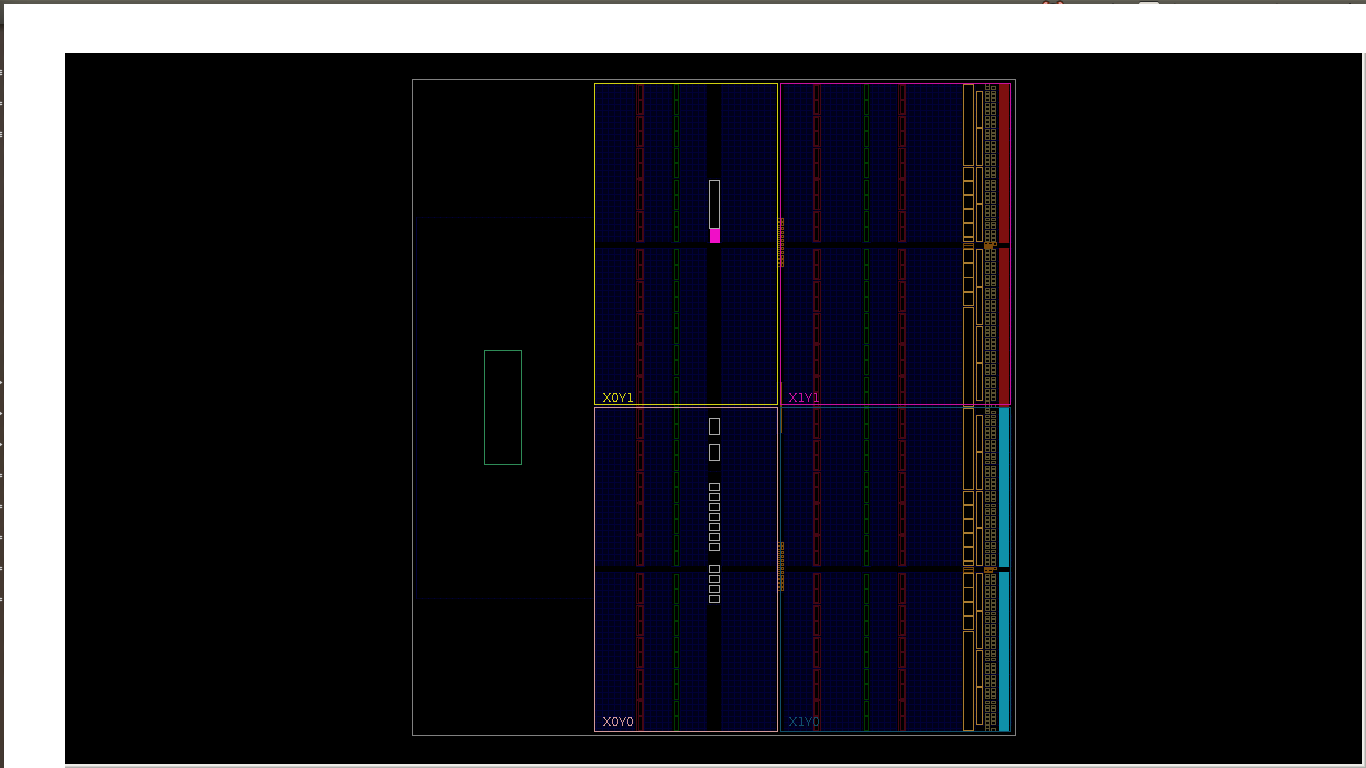
\includegraphics[width=\textwidth, height=8cm]{graphics/fpga_1.png} \\ \\

The resource distribution on the x and y coordinates can be described as \\

\hspace{15mm} \#BRAM \hspace{15mm} h.0 \hspace{10mm}  0$<$x$<$4 
   
   					  \hspace{48mm} h.1 \hspace{10mm}  4$\leq$x$<$18
   					  
   					  \hspace{48mm} h.2 \hspace{10mm}  18$\leq$x$<$25
   					  
   					  \hspace{48mm} h.2 \hspace{10mm}  25$\leq$x$<$W  \\
   					  

\hspace{15mm} \#DSP  \hspace{20mm} h.0 \hspace{10mm}  0$<$x$<$7

					  \hspace{49mm} h.1 \hspace{10mm}  7$\leq$x$<$22
					  
					  \hspace{49mm} h.2 \hspace{10mm} 22$\leq$x$<$W   \\
					  

\hspace{15mm} \#CLB  \hspace{20mm} h.x \hspace{15mm}     0$<$x$<$4
					  				  
					  \hspace{48mm} h.(x-1) \hspace{10mm} 4$\leq$x$<$7
					  
					  \hspace{48mm} h.(x-2) \hspace{10mm} 7$\leq$x$<$10
					  
					  \hspace{48mm} h.(x-3) \hspace{10mm} 10$\leq$x$<$15
					  
					  \hspace{48mm} h.(x-4) \hspace{10mm} 15$\leq$x$<$18
					  
					  \hspace{48mm} h.(x-5) \hspace{10mm} 18$\leq$x$<$22
					  
					  \hspace{48mm} h.(x-6) \hspace{10mm} 22$\leq$x$<$25
					  
					  \hspace{48mm} h.(x-7) \hspace{10mm} 25$\leq$x$<$W
					  
\hspace{15mm} \#static \hspace{48mm} h.x    \hspace{10mm} x = 10 and 15		  
					  
\hspace{15mm} where \[h\in \{0, H-1 \}  \quad and \quad x\in \{0, W-1 \} \] \\

The total number of resources in a slot S(x, y, w, h) = (f(x+w, y+h) - f(x,y)) + (g(x+w, y+h) - g(x,y)) + (k(x+w, y+h) - k(x,y)) where f(x,y), g(x,y) and k(x,y) represent the number CLBs, DSP and BRAM from the bottom left point to (x,y) coordinate on the fpga fabric.

\hspace{15mm} (\textbf{to be included}: the position of the forbidden regions which are going to be used to formulate constraints) \\

The PR constraints used to generate the slot positions are
\begin{itemize}
\item there must be enough resources within the slots
\item A frame can not be shared between two reconfigurable partitions (no interference)
\item forbidden regions must not be included in the slots 
\item Left and right edges must be placed in proper positions
\item the amount of wasted resources should be minimized (Wasting DSPs is more expensive than BRAMs which in turn is more expensive than CLBs)
\item Other optimizations such as lower wire length between slots or lower length to I/O etc... can be added as constraints
\end{itemize}

\textbf{constraint 1}: This is fairly straight forward and needs no further elaboration \\
\textbf{Constraint 2}: A frame (tile) is the smallest reconfigurable physical region and it spans one clock region high and one resource wide. A Reconfigurable Frame cannot contain logic from more than one Reconfigurable Partition. This can be stated as two slots S$_1$ \{x$_1$, y$_1$, w$_1$, h$_1$\} and S$_2$\{ x$_2$, y$_2$, w$_2$, h$_2$ \} do not interfere if \\

\hspace{15mm}  x$_1$ + w$_1$ $<$ x$_2$ or y$_1$ + h$_1$ $<$ y$_2$ : (x$_1$ $<$ x$_2$ and y$_1$ $<$ y$_2$) \\

\textbf{constraint 3}: Global resources, clock resources (central clock column, BUFG, BUFR, MMCM etc...), static components (BSCAN, ICAP, XADC etc...) must not be included in the rectangles. The FPGA resource description must also include the location of these components to prohibit their inclusion in the rectangles

\textbf{constraint 4}: The left and right edges of the rectangles must be placed between CLB-CLB, CLB-BRAM or CLB-DSP and not between two interconnect columns (INT-INT).

\textbf{constraint 5}: This constraint has two parts. The first part states that the slots must be the smallest possible rectangles which contain the required amount of resources. The second part of the constraint states that the number of wasted resources should be kept to the minimum. Resources are considered wasted if they are included in a slot while not being used. All FPGA resources are not equally valuable. This means it is better to waste CLBs than BRAMs than DSPs. Hence there should be some kind of constraint to state the maximum amount of resources that can be wasted in search of an optimal slot. This constraint must also force the optimizer to start searching for slots from the columns of the most expensive resources. \\

\textbf{constraint 6}: Other constraints such as minimal wire length between slots (to reduce routing delay and power consumption) can be used as constraints to choose the optimal slots \\
 
Previous approaches of solving the floorplanning problem by other authors mostly involve two steps. First, all the possible slots are enumerated. This is done by starting a scan on the fpga fabric from the bottom left corner and lisitng all the possible rectangles which will contain all the necessary resources for the respective slots. Then some sort of heuristics/optimization is applied to choose the best ones from the set of possible slots.\\
Our approach instead focuses on using a mathemathical techniques to generate the slots first hand (without enumerating all possible slots) by using the proper constraints. 


The system will finally return the parameters of S$_1$ \{x$_1$, y$_1$, w$_1$, h$_1$\} and S$_2$\{ x$_2$, y$_2$, w$_2$, h$_2$ \} \\


\end{document}